\documentclass{report}
\usepackage{E:/Documents/GitHub/University/LaTeX/marzstyle}

\runningheads{Programming Language}{Exercise 11}

\setcounter{chapter}{11}

\begin{document}
	\section{Using the partition predicate to create a program that ask for a number and creates a lower and greater list from a given list}
	\startsection
	We can define the following rules to define the program:
		\begin{minted}{haskell}
use_module(library(hiordlib)).
partition(E,[],[],[]).
partition(E,[H|T],[H|T1],L2) :- H < E, partition(E,T,T1,L2).
partition(E,[H|T],L1,[H|T2]) :- H > E, partition(E,T,L1,T2).
		\end{minted}
	\closesection
	
	\section{Create a finite collecton of definite clause grammar rules to check whether a sentence is grammatically correct.}
	\startsection
		\begin{minted}{haskell}
article --> [a].
article --> [the].
noun --> [girl].
noun --> [boy].
pronoun --> [that].
pronoun --> [this].
auxiliary --> [is].
verb --> [sleeps].
verb --> [likes].

subject --> article, noun.
subject --> pronoun.
subject1 --> article, noun.
predicate --> auxiliary.
predicate --> verb.
object --> article, noun.

sentence --> sp.
sentence --> spo.
sp --> subject, [sleeps].
spo --> subject1, [likes], object.
spo --> pronoun, auxiliary, object.
		\end{minted}
		So for testing purposes we get the following output (https://swish.swi-prolog.org/):
		\begin{center}
			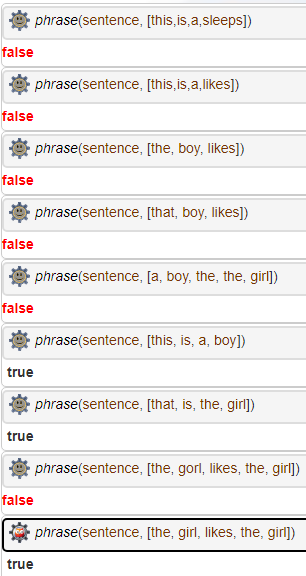
\includegraphics[scale=0.42]{Prolog_Execution.png}
		\end{center}
	\closesection
\end{document}